\documentclass[border=10pt]{standalone}
\usepackage{pgfplots}
\pgfplotsset{compat=1.18}
\begin{document}
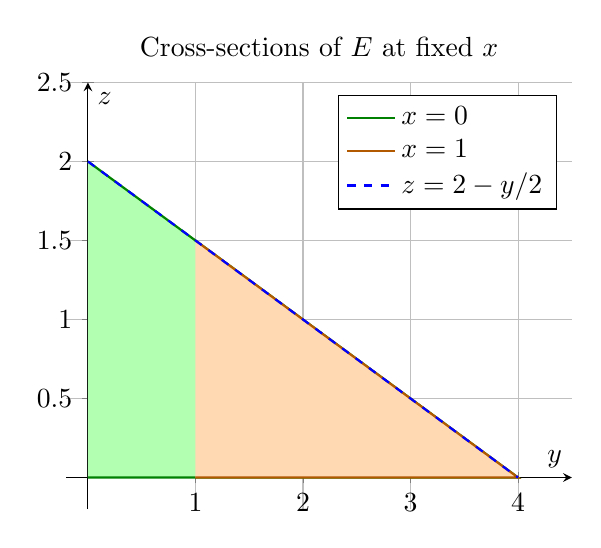
\begin{tikzpicture}
\begin{axis}[
    width=8cm, height=7cm,
    xlabel=$y$, ylabel=$z$,
    xmin=-0.2, xmax=4.5,
    ymin=-0.2, ymax=2.5,
    axis lines=middle,
    grid=both,
    title={Cross-sections of $E$ at fixed $x$},
    legend pos=north east,
    legend cell align=left,
]
\addplot[fill=green!30, draw=green!50!black, thick] coordinates {(0,0) (4,0) (0,2)};
\addlegendentry{$x=0$}
\addplot[fill=orange!30, draw=orange!70!black, thick] coordinates {(1,0) (4,0) (1,1.5)};
\addlegendentry{$x=1$}
\addplot[blue, dashed, thick, domain=0:4, samples=100] {2-x/2};
\addlegendentry{$z=2-y/2$}
\end{axis}
\end{tikzpicture}
\end{document}